\chapter{Introduction}
\label{chap:intro}
\tightlists
% Intro: slightly more than 30 pages in a review form, and set up framework (topics and challenges) for the projects

% Cancer
% mutation
% Multi-omics

% PTM
% heterogeneity
% tumor microenvironment
% precision medicine


% Large scale patient samples collection (consoritum works)

% data portal

% data sharing
% pipeline execution
% gene annotation
% integration


% GBM

% Outline of the dissertation


\section{Cancer and precision medicine}
Cancer is the leading cause of death in most countries in the world \cite{sungh_brayf:GlobalCancer2021}. In the U.S., cancer is estimated to introduce roughly 1.9 millions cases and 600 thousands deaths in 2021, where \textasciitilde40\% of the population will be diagnosed with cancer at some point in their lifetime \cite{siegelrl_jemala:CancerStatistics2021}. Despite advancements in understanding and treating cancer in the past 50 years, many forms of the disease lack effective treatment, and how normal cells become cancerous and form a tumor, the process known as oncogenesis, remains to be fully deciphered. Therefore, the cancer research community continues to work on better characterization of cancer and its treatment as our ultimate goals.

The functional properties of a tumor have been described as ``cancer hallmarks'' \cite{hanahand_weinbergra:HallmarksCancer2011}, including cell proliferation, immortality in replication, cell death evasion, and increased ability of angiogenesis and invasion. While the tumor microenvironment, the surrounding tissue environment where a tumor develops, consists of normal cells, the tumor microenvironment also helps maintain tumor abberrant growth and immune respones beneficial to the tumors \cite{hanahand_weinbergra:HallmarksCancer2011,quaildf_joyceja:MicroenvironmentalRegulation2013}. To develop an effective cancer treatment, it's important to understand how cancer hallmarks are achieved during oncogenesis and the complicated cell-cell interactions in the tumor microenvironment.


\subsection{Oncogenesis and the functional impact of somatic mutation}
Oncogenesis is currently viewed as a microevolution process where normal cells acquire somatic mutations that offer growth and survival advantage \cite{strattonmr_futrealpa:CancerGenome2009,martincorenai_campbellpj:SomaticMutation2015}. The somatic mutation rate in human is estimated to be about 2 to 10 mutations per cell division \cite{lynchm_lynchm:RateMolecular2010,milhollandb_vijgj:DifferencesGermline2017}. A tumor may accumulate 0.01--100 mutations per megabase in the genome depending on the cancer type \cite{lawrencems_getzg:MutationalHeterogeneity2013,martincorenai_campbellpj:SomaticMutation2015}. However, only some of the mutations might confer a growth and survival advantage while remaining mutations are either benign or of unknown phenotype. Such actively selected mutations are frequently found in certain genes, known as cancer driver genes or significantly mutated genes (SMGs) \cite{dingl_mariamidzea:PerspectiveOncogenic2018}. There are three main types of cancer driver genes: proto-oncogenes that promotes cell growth, tumor suppressor genes that regulate cell growth, and DNA rapair genes that fix DNA damages.

Mutations in one cancer gene or a combination of them are sufficient to drive the oncogenic process. For example, transcription factor \gene{TP53} is a tumor suppressor gene\footnotemark{} and it responds to DNA damage by inducing cell cycle arrest \cite{kastanmb_craigrw:ParticipationP531991}. Mutations in TP53 can lead to the uncontrolled proliferation of mutated cells, thereby causing cancer. Thus, \gene{TP53} is one of the most commonly found cancer genes in a tumor, whose mutations can be found in a remarkable 37.5\% of over 9 thousands tumor samples examined across 33 cancer types \cite{baileymh_dingl:ComprehensiveCharacterization2018}. On the other hand, \gene{EGFR}, epidermal growth factor receptor, is a well known proto-oncogene that encodes a transmembrane protein that activates cell signaling pathways to promote cell growth. The mutations in \gene{EGFR} often lead to increased gene expression or uncontrolled activation of its function, and are commonly found in breast, lung, and brain cancer patients \cite{ciardiellof_tortorag:EGFRAntagonists2008}.

\footnotetext{\gene{TP53}'s role as a cancer drive gene is complicated. While the majority of its mutations are loss-of-function, leading to decreased ability to suppress tumor growth, it also exhibits oncogene properties with gain-of-function mutations \cite{petitjeana_olivierm:TP53Mutations2007}.}

Therefore, characterizing the functional impact of a mutation has been an area of intensive research ever since the first cancer somatic mutation was identified in \citeyear{reddyep_barbacidm:PointMutation1982} \cite{reddyep_barbacidm:PointMutation1982,tabincj_changeh:MechanismActivation1982}. Besides well controlled experimental validation, a number of statistical methods have been widely-used to infer functional elements, including high gene mutation rate, mutation recurrence, mutual exclusivity, and co-occurrence of mutations across multiple samples or cancer types, since these phenomena imply positive selection \cite{martincorenai_campbellpj:SomaticMutation2015}. However, only a few mutations are well understood and the majority of them have unknown function in cancer. Even for well-known cancer driver genes like \gene{PIK3CA} and \gene{BRCA1/2}, only a fraction of suspected cancer-related mutations having actually been functionally validated \cite{ngpks_millsgb:SystematicFunctional2018}. It is still challenging today to attribute a phenotypic ``cancer hallmark'' expressed by a tumor to its mutations.


\subsection{Multi-omics portrait of cancer}
Since the phenotypes of cancer hallmarks are achieved through abberant alterations at multiple molecular levels, a new paradigm to understand complex diseases like cancer is through the lens of multi-omics analysis \cite{deanda-jaureguig_hernandez-lemuse:ComputationalOncology2020}. Thanks to the recent advancements in high-throughput experiments (commonly termed ``omics''), we are able to profile the specimen systematically at a molecular level. Common omics assays include:

\begin{itemize}
    \item Genomic: whole exome sequencing, whole genome sequencing
    \item Transcriptome: RNA sequencing, miRNA sequencing
    \item Epigenomics: DNA methylation microarray, whole genome bisulfite sequencing, ChIP-seq, ATAC-seq
    \item Proteomics: TMT multiplexed mass spectrometry
    \item Single cell omics: single cell/nuclei RNA and ATAC sequencing
    \item Imaging: Imaging mass cytometry, CODEX, histopathology H\&E slides
    \item Spatial transcriptomics: 10x Genomics Visium
\end{itemize}

By investigating the biological signals and features accquired from different molecular assays in the same specimen, we are able to ``connect the dots'' and reason how a genetic alteration contributed to the phenotypes, furthermore, how a set of genetic alterations interact together. For example, \gene{EGFR} is an oncogene commonly altered in glioblastoma \cite{eskilssone_miletich:EGFRHeterogeneity2018}, but we are unsure of its functional impact. Using multi-omics approaches, we will be more confident to attribute the cell profileration of a glioblastoma to genetic alterations in \gene{EGFR} if we are able to pick up concordant findings from different experiment assays: mutation or amplification of \gene{EGFR} is detected; RNA expression, protein abundance, and activating phosphorylation of EGFR are all increased in this sample relative to the wild-type tumors and normal samples; increased activity in the RTK-RAS-MAPK pathway; single cell and imaging omics showing the increased EGFR activity is found in tumor cells and not normal cells in the tumor microenvironment. Multi-omics analysis allows us to model the complex biological phenomenon as systems consisting of complicated interactions, which allows us to protray the relatively abstract activities of cancer hallmarks by mapping all the abberant activities simultaneously.

Conducting multi-omics characterization of cancer naturally calls for large scale collaborations since it requires more samples to power statistical modeling and requires different expertise to carry out diverse experimental assays and data integration. As a result, more consortia and large-scale projects are founded as the foundation for multi-omics studies \cite{hutterc_zenklusenjc:CancerGenome2018,rozenblatt-roseno_zhuangx:HumanTumor2020,rodriguezh_lowydr:NextHorizon2021}.


\subsection{Precision medicine}

% Due to the random nature of oncogenesis, each tumor is different in their mutational profile.


% Our lab has also studied the effect of coding mutations on protein structure \cite{niu_protein-structure-guided_2016}. \citeauthor{niu_protein-structure-guided_2016} found that mutations cluster spatially in the functional protein domains of driver genes. For example, mutations clustering near an EGFR phosphotyrosine site in the 3D tertiary structure have been shown to increase autophosphorylation levels and EGFR activity \cite{niu_protein-structure-guided_2016}.

% Many somatic mutations have unknown significance; transition to PTM
%  Since post-translational modifications (PTMs) are known to be essential for signal transduction \cite{hunter_signaling2000_2000}, I propose to explore the functional impacts of mutations by investigating their effects on PTMs.


% TODO: need a section to describe TCGA, CPTAC and HTAN

\section{Computational challenges in large-scale multi-omics studies}
Large scale multi-omics studies produce massive amounts of data, providing insights into complicated biological systems and allowing researchers to generate hypotheses from their research angle. However, they also introduce a new set of computational challenges that impede the utility of the data \cite{marxv_marxv:DrillingBig2013,deanda-jaureguig_hernandez-lemuse:ComputationalOncology2020}, which can be summarized into the four foundational principles using FAIR guideline: Findability, Accessibility, Interoperability, and Reusability \cite{wilkinsonmd_monsb:FAIRGuiding2016}. In this study, we focus on the data harmonization and annotation cross-reference.


\subsection{Data harmonization on centralized repositories}
The Cancer Genome Atlas (TCGA) \cite{hutterc_zenklusenjc:CancerGenome2018} and the International Cancer Genomics Consortium (ICGC) \cite{internationalcancergenomeconsortium_yangh:InternationalNetwork2010} are among the early large scale cancer multi-omics studies that collected genomic, transcriptome, and epigenomic data from tens of thosands patients. Theses studies then developped their data repositories to accommodate and process their multi-omics datasets, including NCI Genomics Data Commons (GDC)\footnotemark{} \cite{heathap_grossmanrl:NCIGenomic2021} and ICGC Data Portal \cite{jolyy_chalmersd:DataSharing2012}. To date (2012), GDC has included 13 different cancer genomic programs and has become the \textit{de facto} cancer genomics data repository. With the success of GDC, a bigger framework of ``Data Commons'', NCI Cancer Research Data Commons (CRDC) \cite{hinksoniv_kibbewa:ComprehensiveInfrastructure2017}, has been proposed to provide data repositories for other data types and they are under active development:
\begin{itemize}
    \item Proteomic Data Commons: \url{https://pdc.cancer.gov/pdc/}
    \item Imaging Data Commons: \url{https://portal.imaging.datacommons.cancer.gov/}, superceding The Cancer Imaging Archive (TCIA) \url{https://www.cancerimagingarchive.net/}
\end{itemize}

\footnotetext{
    There are a few precursor initiatives before NCI GDC to harmonize and process the TCGA datasets. For example, Firehose developed by Broad Institute's Genome Data Analysis Center (GDAC) \cite{marxv_marxv:DrillingBig2013} has been processing TCGA datasets using standardized pipelines. See \url{https://gdac.broadinstitute.org/} and \url{https://broadinstitute.atlassian.net/wiki/spaces/GDAC/}. The Firehose results are released with tracked and document version, which laid the foundation of the infrastructure design for future projects like GDC.
}

To allow comparison and integration between different datasets, a set of standardized pipelines are developed by GDC to process all the raw data uniformly \cite{zhangz_grossmanrl:UniformGenomic2021}. The pipelines cover typical genomics data, including whole exome sequencing (WXS or WES), whole genome sequencing (WGS), RNA-Seq, and DNA methylation microarray. The pipelines specifies the tool, version, and parameters for sequence alignment and further downstream processing that are applied the same to every sample in the data repository. The pipelines are designed to handle various sequencing artifact and combine the best practices known to the research community. For example, the genome reference (GRCh38.d1.vd1) contains human decoy sequences and cancer related virus genomes (e.g. Cytomegalovirus [CMV], Epstein-Barr virus [EBV], Hepatitis B virus [HBV], Hepatitis C virus [HCV], and Human immunodeficiency virus [HIV]) to improve the sequence alignment quality \cite{zhangz_grossmanrl:UniformGenomic2021}. The WES somatic mutation calling pipeline built on the evolving best practices throughout the development of TCGA and ICGC-TCGA Dialogue for Reverse Engineering Assessments and Methods (DREAM) challenges \cite{ewingad_boutrospc:CombiningTumor2015,ellrottk_tcga:MC3MutationCalling2018}. The pipeline implements various annotations and filtering to improve the mutation calling, including a panel of normal samples to filter false-positive, contamination, and germline variants; 8-Oxoguanine (OxoG) DNA lesion introduced by the excessive oxidation during the sequencing library preparation; contamination removal.

However, the data harmonization ultimately changes the final output of the genomic pipelines, which might introduce unknown technical artifacts and biases that might affect the downstream biological interpretation. While such differences can be spotted by comparing the outputs on the same input sequence data, it is difficult to explain the differences due to the complicated implementation (e.g. the reason a mutation is called or filtered). Non-trivial efforts are required to characterize the pipeline differences and summarize in less technical terms.


\subsection{Annotation difference}
% Data management
% gene annotation difference
%     gene symbol
%     gene version
%     annotation across different data types


Gene naming \cite{fujiyoshik_oginos:OpinionStandardizing2021, brufordea_tweedies:GuidelinesHuman2020} \tref{tab:intro-anno}

\begin{SingleSpace}
\begin{table}[tbp]
    \centering
    \caption{Comparison of commonly used annotations.}
    \label{tab:intro-anno}

    \footnotesize
    \begin{subtable}{1\linewidth}
        \centering
        \subcaption{Gene level}\label{tab:intro-anno-gene}
        \begin{tabular}{lllp{15em}}
            \toprule
            Identifier      & Example   & Sequence  & Notes \\
            \midrule
            Gene symbol     & EGFR      & -         &
            \begin{tablist}
                \item Biologically meaningful name
                \item Often change over time
            \end{tablist}\\
            HUGO Gene ID    & HGNC:3236 & -         &
            \begin{tablist}
                \item Stable
                \item IDs can be deprecated
            \end{tablist}\\
            Ensembl         & ENSG00000146648\textbf{.20} & - &
            \begin{tablist}
                \item Stable
            \end{tablist} \\
            NCBI Entrez	    & 1956      & -         &
            \begin{tablist}
                \item Stable
                \item Difficult to cross-reference
            \end{tablist} \\
            \bottomrule
        \end{tabular}
    \end{subtable}

    \vspace{0.5\baselineskip}
    \begin{subtable}{1\linewidth}
        \centering
        \subcaption{Transcript level}\label{tab:intro-anno-transcript}
        \begin{tabular}{lllp{15em}}
            \toprule
            Identifier      & Example           & Sequence   & Notes \\
            \midrule
            Ensembl         & ENST00000275493\textbf{.7}    & Stable &
            \begin{tablist}
                \item Recommended
                \item Wildly in use
            \end{tablist}\\
            RefSeq          & NM\_005228\textbf{.5}         & Stable &
            \begin{tablist}
                \item Lack stable genomic location
                \item Lack batch release
            \end{tablist}\\
            \bottomrule
        \end{tabular}
    \end{subtable}

    \vspace{0.5\baselineskip}
    \begin{subtable}{1\linewidth}
        \centering
        \subcaption{Protein level}\label{tab:intro-anno-protein}
        \begin{tabular}{lllp{15em}}
            \toprule
            Identifier      & Example           & Sequence   & Notes \\
            \midrule
            Ensembl         & ENSP00000275493\textbf{.2}    & Stable &
            \begin{tablist}
                \item Redundant
            \end{tablist}\\
            RefSeq          & NP\_005219\textbf{.2}         & Stable &
            \begin{tablist}
                \item Non-redundant
                \item Lack batch release
            \end{tablist}\\
            UniProt         & P00533\textbf{.v2}            & Unstable &
            \begin{tablist}
                \item Non-redundant
                \item Wildly in use
                \item Rich metadata
                \item Hidden versioning
                \item Lack genomic location
                \item Hard to work on old releases
            \end{tablist}\\
            UniProt isoform & P00533\textbf{-1.v2}          & Stable &
            \begin{tablist}
                \item Rarely in use
            \end{tablist}\\
            UniParc         & UPI000003E750                 & Stable &
            \begin{tablist}
                \item Non-redundant
                \item Permanent
                \item Rarely in use
                \item Hard to cross-ref to transcripts
            \end{tablist}\\
            \bottomrule
        \end{tabular}
    \end{subtable}
\end{table}
\end{SingleSpace}


\subsection{Unaccounted batch effects}
In this section, we focused on studies that have a standardized set of experiment techniques and protocols. However, there are additional obstacles in integrating data of the same molecular type but by different protocols. For example, RNA-seq using polyA enriched and ribosomal RNA depletion protocols captures different RNA species and may different variations in the expression quantification \cite{cuip_yuj:ComparisonRibominus2010,chenl_chenl:PairedRRNAdepleted2020}. Phosphoproteomics generated by different mass spectrometry strategies (e.g., MS2 and MS3 spectra) have greatly variable ability to identify phosphopeptides and different dynamic ranges in the quantification \cite{ulintzpj_nesvizhskiiai:ComparisonMS2only2009}. The existing data repositories like GDC and SRA do not automatically remove the batch effect introduced by the different experiment protocols, so it is up to the users to apply extra care and computational approaches to determine the severity of such batch effect and the approach of batch effect removal.



\section{Post-Translational modifications (PTM) in cancer}
Post-translational modifications (PTMs) dynamically regulate protein function through the covalent addition of chemical moieties to nascent polypeptides following translation. More than 200 known PTM types have been identified \cite{deribeyl_dikici:PosttranslationalModifications2010}. Post-translational proteolysis is a PTM that involves cleavage of peptides. Common examples include the removal of initial methionine (N-terminal methionine excision) \cite{giglionec_meinnelt:ProteinNterminal2004} and the removal of some signal peptides, short peptides at N-terminus, necessary for protein translocation \cite{martogliob_dobbersteinb:SignalSequences1998}. Disulfide-bond formation between two cysteine residues is another form of PTM that involves more than on residues and helps stabilize protein structure \cite{wedemeyerwj_scheragaha:DisulfideBonds2000}. Post-translational modifications are necessary for the maturation of many proteins. For example, human insulin requires peptide trimming, signal peptide removal, and formation of disulfide bonds to fold into its correct structure. Other PTMs affect amino acid side chains and generally play an important role in cell signaling or gene regulation. Common PTMs in this category include phosphorylation, ubiquitination, acetylation. Notably, phosphorylation of adaptor proteins by kinases can potentiate intracellular signaling, while histone acetylation by acetyltransferases can affect chromatin architecture. Alternatively, lysine polyubiquitination by ubiquitin ligases can promote proteasomal degradation of substrate proteins. In my thesis, we will focus on these three PTMs and their function in cancer.


\subsection{The role of phosphorylation in signaling pathways}
Phosphorylation is the most common PTM in human cells and it occurs mostly on serine (61.8\%), threonine (24.0\%), and tyrosine (14.2\%) residues \cite{hornbeckpv_sullivanm:PhosphoSitePlusComprehensive2012}. Kinases are enzymes that add a phosphoryl group to an amino acid. Phosphorylation is reversible by enzymes called phosphatases, which catalyze the removal of phosphoryl group. Phosphorylation on other residues are also possible, including histidine, arginine, and lysine, though such PTMs are uncommon in mammalian cells \cite{whitefm_wolf-yadlina:MethodsAnalysis2016}.

% The function of protein kinases and phosphatases
Phosphorylation plays an important role in human cell signal transduction. During signal transduction, a chemical or physical signal is transmitted to a cell through a series of molecular reactions, typically catalyzed by protein kinases. For example, cyclin-dependent kinases (CDKs) can regulate the cell cycle with the presence of different cyclin proteins \cite{malumbresm_malumbresm:CyclindependentKinases2014}. In particular, CDK4 proteins drive the cell cycle transition from G1-phase to S-phase when D-type cyclin proteins are present \cite{olearyb_turnernc:TreatingCancer2016}. The activated cyclin D-CDK4 complex subsequently phosphorylates retinoblastoma protein pRb \cite{narasimhaam_dowdysf:CyclinActivates2014}. Unphosphorylated or hypophosphorylated pRb binds to the E2F transcription factor (TFs) family proteins, preventing E2F TFs from promoting expression of the genes responsible for S-phase activation and DNA replication. Thus, phosphorylated pRb by CDK4 or CDK6 will release E2F TFs and lead to the cell cycle progression. On the other hand, phosphatases also regulate the cell signaling by removing existing phosphorylated residues. For example, protein phosphatase 1 and 2 (PP1 and PP2A) regulated pRb activity by competing with CDK proteins at the same docking site \cite{wlodarchakn_xingy:PP2AMaster2016}. Through the dynamics of kinase and phosphatase activity, cell signaling pathways are highly regulated and coordinated by phosphorylation.


\subsection{Acetylation and their function}
Acetylation adds an acetyl group to either the N-terminal of proteins or a lysine residue. N-terminal acetylation is catalyzed by N-terminal acetyltransferases (NATs) co-translationally on the majority of human proteins \cite{starheimkk_arnesent:ProteinNterminal2012}. This irreversible reaction is not the main focus of this study. The other type of acetylation occurs post-translationally by transferring the acetyl group from acetyl-coenzyme A (acetyl-CoA) to the ε-amine of a lysine residue \cite{alii_ottm:LysineAcetylation2018}. Lysine acetylation is reversible and its function involve three types of proteins: ``writers'' of lysine acetyltransferases (KATs) that introduce the acetylation, ``erasers'' of lysine deacetylases (KDACs) that remove the acetylation, and ``readers'' of proteins with specific acetyl-lysine binding domains that recognize acetylation sites.

Histone acetylation is a well-studied epigenetic mark involved in transcriptional regulation \cite{shahbazianmd_grunsteinm:FunctionsSiteSpecific2007,alii_ottm:LysineAcetylation2018}. Histone acetylation has been shown in yeast to remodel the chromatins at the promoter region of active genes \cite{suganumat_workmanjl:SignalsCombinatorial2011}. Spt-Ada-Gcn5 acetyltransferase (SAGA) or NuA4 complexes can acetylate the N-terminal tails of H2 and H3 histones \cite{hassanah_workmanjl:HistoneAcetyltransferase2001}. A nucleosome remodeling complex SWI/SNF tethers to the acetylated histone by its Swi2/Snf2 subunit with a bromodomain, a common protein domain functioning as the "reader" of the acetylated lysine \cite{awads_hassanah:Swi2Snf22008}. SWI/SNF complex then displaces the DNA from the acetylated histones and creates a nucleosome-free region, enabling the promoter region accessible for the gene activation \cite{awads_hassanah:Swi2Snf22008}.

The role of lysine acetylation on proteins other than histones has also been investigated. For example, CBP (\gene{KAT3A}) and p300 (\gene{KAT3B}) acetylate and activate p53 by promoting its DNA-binding ability \cite{scolnickdm_halazonetistd:CREBbindingProtein1997,brookscl_guw:ImpactAcetylation2011}. On the other hand, p53 can be deacetylated and inactivated by KDACs such as sirtuin 1 (\gene{SIRT1}) and HDAC1 \cite{brookscl_guw:ImpactAcetylation2011,luoj_guw:DeacetylationP532000}. Therefore, the activity of transcription factors like p53 can be regulated by the dynamics of both KATs and KDACs through acetylation.


\subsection{Ubiquitination and their function}
Ubiquitination adds a small protein, ubiquitin, to a lysine residue of a protein substrate. The main function of ubiquitination is to mark the substrate for degradation by the proteasome \cite{komanderd_rapem:UbiquitinCode2012}. Ubiquitination is also capable of altering the cellular location of a substrate \cite{mukhopadhyayd_riezmanh:ProteasomeIndependentFunctions2007} and its function \cite{schnelljd_hickel:NontraditionalFunctions2003}. A full process of ubiquitination involves three major steps: activation, conjugation, and ligation, each with a corresponding set of proteins. Starting with the activation step, the ubiquitin-activating enzyme E1 creates a covalent bond with a ubiquitin and activates the ubiquitin. At the conjugation step, the ubiquitin-conjugating enzyme E2 catalyzes the transfer of the activated ubiquitin from E1 to E2 itself. Finally, at the ligation step, the ubiquitin ligase E3 recognizes both E2 and the targeting lysine residue on the substrate and introduces an isopeptide bond between the lysine and the ubiquitin from E2. Ubiquitination is reversible by deubiquitinating enzymes (DUBs), which either completely or partially remove the attached ubiquitins from the substrate protein \cite{reyes-turcufe_wilkinsonkd:RegulationCellular2009}.


\subsection{Methylation and their function}
Protein methylation adds a methyl group to the protein substrate by methyltransferase, and predominantly affects lysine and arginine residues \cite{murnj_shiy:WindingPath2017}. Unlike other PTMs, lysine and arginine can accept up to three or two methyl groups respectively at the same residue, forming mono-, di-, and tri-methylation. Methylation is also a reversible modification which can be "erased" by demethylases.

Histone methylation is considered another important epigenetic histone mark associated with transcription regulation. The location and the degree of the methylation of a methyl-lysine residue on the histone tail changes the effect on gene expression \cite{greerel_shiy:HistoneMethylation2012}. For example, H3K4me3 is commonly correlated with an active transcript of the adjacent gene. Nucleosome remodeling factor (NURF) recognizes the methylated histone with its PHD finger domain and initiates chromatin remodeling \cite{wysockaj_alliscd:PHDFinger2006}. Conversely, H3K27me3 is associated with an inactive gene promoter, which may be the result of methylation and acetylation competing for the same lysine residue \cite{pasinid_helink:CharacterizationAntagonistic2010}. Histone methylation sites are also shown to be maintained across cell divisions, though the underlying mechanism remains elusive \cite{greerel_shiy:HistoneMethylation2012}. Outside of histone methylation, arginine methylation has been shown to regulate the activity of RNA-binding proteins (RBPs) \cite{murnj_shiy:WindingPath2017}.


\subsection{PTM substrate recognition shows local sequence preference}
% Linear specificity
Many PTM related enzymes have an evolutionarily conserved substrate binding domain which exhibits strong preference for a specific amino acid sequence proximal to the residue \cite{manningg_sudarsanams:ProteinKinase2002, taylorss_kornevap:ProteinKinases2011,endicottja_johnsonln:StructuralBasis2012,chenmj_manningg:GenomicsEvolution2017,ochoad_beltraop:EvolutionDynamics2018,alii_ottm:LysineAcetylation2018}. In other words, a mutation proximal to a PTM site can affect how PTM-related enzymes recognize the site, which may affect PTM abundance and its downstream function. For example, human kinases can be clustered by their sequence similarities in the kinase domain into 9 large kinase groups and 134 kinase families \cite{manningg_sudarsanams:ProteinKinase2002}. All kinases have a similar two-lobe structure and contain the P+1 loop to accommodate the +1 residue of the substrate peptide \cite{taylorss_kornevap:ProteinKinases2011}. This sandwich-like structure offers both high specificity and flexibility to be regulated by upstream signaling \cite{taylorss_kornevap:ProteinKinases2011}. For example, cyclin-dependent kinases (CDKs) prefer \textbf{S/T}-P-X-K/R substrate sequences \cite{endicottja_johnsonln:StructuralBasis2012,ochoad_beltraop:EvolutionDynamics2018}. Many other kinase families also exhibit substrate specificity between P-6 to P+6 amino acids \cite{hornbeckpv_skrzypeke:PhosphoSitePlus2015}. The SH2 protein domain, a well-studied domain that binds to phosphotyrosine, shows high affinity only to a subset of all possible P+1 to P+3 amino acid sequences \cite{zhous_cantleylc:SH2Domains1993}. Similar structure conservation and substrate sequence specificity are also observed in other PTMs. Non-histone acetylated lysine substrates have been found to be surrounded by small amino acids and commonly preceded by a glycine residue \cite{basua_hakesb:ProteomewidePrediction2009,schwartzd_churchgm:PredictingProtein2009}. The substrate specificity of some methyltransferases has also been characterized, such as methyltransferase G9a \cite{rathertp_jeltscha:ProteinLysine2008,hameyjj_wilkinsmr:MTMAMSProtein2018}, protein arginine N-methyltransferase 1 \cite{hameyjj_wilkinsmr:MTMAMSProtein2018}, and SET7/9 \cite{dhayalana_jeltscha:SpecificityAnalysisbased2011}.

% Structural specificity
The ``sequence proximity'' of PTM substrate specificity should also be investigated in three-dimensional space. A mutation distal to a PTM site on the linear protein sequence may be spatially close to the site on the protein structure. Although substrate specificity through 3D structure remains elusive for most PTM enzymes, studies have shown that modeling substrate preference through linear sequence is grossly insufficient. For example, PKC kinase shows spatial substrate specificity that its linear motif is unable to capture \cite{duarteml_schechtmand:ProteinFolding2014}. Our lab has also found experimentally that the cancer mutations clustered spatially around a EGFR phosphotyrosine are associated with higher autophosphorylation and protein expression \cite{niub_dingl:ProteinstructureguidedDiscovery2016}.


\subsection{Examples of proximal mutations affecting PTM functions in cancer}
\begin{figure}[tb]
    \centering
    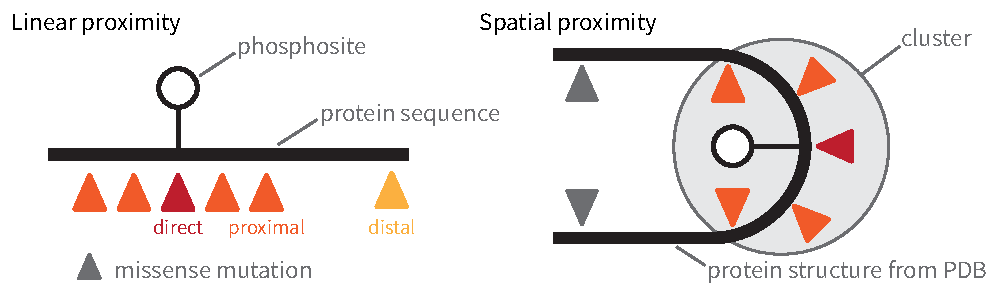
\includegraphics[width=0.9\linewidth]{figures/chap01_intro/ptm_mutational_impact.pdf}
    \caption{Schematic overview of mutational impact on PTM function.}
    \label{fig:intro-ptm-mut-impact}
\end{figure}

% Direct overlap example
Due to the important role of PTMs in cellular signaling, their functions are often perturbed or disrupted in cancer through mutation (\fref{fig:intro-ptm-mut-impact}). The most straightforward effect of a mutation is through its direct overlap with a PTM site on the substrate. The substituted amino acid may not be recognized by the original PTM modifier or might not be modified at all, thus disrupting PTM function. For example, beta-catenin, encoded by \gene{CTNNB1}, is an essential protein in the Wnt signaling pathway regulating cell growth \cite{gaoc_zhangw:ExonMutations2017}. Phosphorylation on its N-terminal domain by GSK3β kinase is required for its degradation via the ubiquitin proteasome pathway \cite{millerjr_moonrt:SignalTransduction1996}. However, hotspot mutations of \gene{CTNNB1} at the N-terminal phosphosites such as S33 and S37 are found in colon, lung, and liver cancers \cite{gaoc_zhangw:ExonMutations2017}. Those mutations potentially disrupt phosphosite-dependent degradation and lead to aberrantly high expression of beta-catenin and uncontrolled cell proliferation.

% Proximal overlap example
A mutation can also substitute the proximal residue of a PTM site, leading to a different PTM abundance level or downstream function change in cancer. For example, aurora kinase B (\gene{AURKB}), a substrate of P-2 arginine \cite{endicottja_johnsonln:StructuralBasis2012}, phosphorylates p53 at the T284 residue and marks p53 for degradation through the ubiquitin proteasome pathway \cite{gullycp_leemh:AuroraKinase2012}. A recurrent mutation in colorectal cancer, \gene{TP53} p.R282W, which changes residue 282 from arginine to tryptophan, has been shown in cell lines to disrupt the T284 phosphorylation by \gene{AURKB} \cite{wagiho_badergd:MIMPPredicting2015}.

To demonstrate the potential impact of mutation and PTM spatial clustering, We developed a tool, HotPho, specifically looking for clusters of mutation and phosphosites on protein structures and identified potentially functional clusters across 5 cancer types \cite{huangk_dingl:SpatiallyInteracting2021}. Taken together, PTM overlapping mutations in cancer have been experimentally shown to disrupt PTM function and abundance. However, PTM abundance was not directly measured in the original cancer samples in the examples above, and the extent of the downstream impact of PTM overlapping mutations is not well understood. By measuring the PTM abundance, gene expression, protein expression, and the mutation profile of the same cancer sample, we will be able to directly observe the PTM overlapping mutations, their impact on a PTM site, and their implication in downstream functions.


\subsection{Large-scale proteomics cancer cohorts by CPTAC}
The Clinical Proteomic Tumor Analysis Consortium (CPTAC) aims to understand the proteogenomic basis of cancer and to accelerate the translation of findings into clinical applications \cite{rodriguezh_lowydr:NextHorizon2021}. CPTAC expands the multi-omics landscape of TCGA to proteins and protein modifications, generating somatic mutation calls, protein expression data, and PTM abundances in paired normal and tumor samples from multiple cancer types. To ensure that the proteomics technology is ready to answer biological questions in a large number of samples, CPTAC has been developed in multiple phases. In the first phase, studies were conducted to evaluate the reproducibility of various mass spectrometry based assays between clinical samples from multiple laboratories \cite{addonata_carrsa:MultisiteAssessment2009,rudnickpa_steinse:PerformanceMetrics2010}. Results showed that mass spectrometry data were reproducible and a strategy was developed to combine the protein and phosphoprotein expressions of multiple experiment runs, allowing the technology to analyze larger sample cohorts. During the second phase of CPTAC, clinical samples of three cancer types were characterized by mass spectrometry assays: colon/rectal cancer (CO) \cite{zhangb_thencicptac:ProteogenomicCharacterization2014}, breast (BRCA) cancer \cite{mertinsp_ncicptac:CPTACBreastCancer2016}, and ovarian cancer (OV) \cite{zhangh_townsendrr:IntegratedProteogenomic2016}. Building upon genomic understanding from previous TCGA studies, CPTAC2 showed the downstream functional impact of the mutations on protein activity in various signaling pathways.

The third and current CPTAC phase, CPTAC3, is exploring the proteogenomic landscape of additional cancer types: clear cell renal carcinoma (ccRCC) \cite{clarkdj_zhangh:IntegratedProteogenomic2019}, uterine corpus endometrial carcinoma (UCEC) \cite{douy_zhaog:CPTACUCEC2020}, lung adenocarcinoma (LUAD) \cite{vasaikars_cptac:ProteogenomicAnalysis2019}, glioblastoma (GBM) \cite{wanglb_cptac:GBM2021}, pancreatic adenocarcinoma (PDAC) \cite{caol_zhaog:ProteogenomicCharacterization2021}, lung squamous cell carcinoma (LSCC) \cite{satpathys_hanhanz:ProteogenomicPortrait2021}, head and neck squamous cell carcinoma (HNSCC) \cite{huangc_zhuj:ProteogenomicInsights2021}, and more. For each cancer type, CPTAC3 will collect around 200 treatment-naive samples and split these samples into discovery and confirmatory cohorts. Besides the phosphoproteome data that previous CPTAC cohorts have generated, studies of many CPTAC cancer types will also provide other PTM enriched MS data, including acetylation, ubiquitination, methylation, and glycosylation.



\section{Glioblastoma}
GBM is the most common primary malignant brain tumor with an incidence of 3.22 per 100,000 persons in the United States, a median survival of less than 2 years from diagnosis18,19 and limited treatment options20,21. TCGA surveyed 206 GBMs with genomic and transcriptomic profiling22, extending the subclassifications developed by Aldape and colleagues23,24. The current view is that IDH-wild type GBMs fall into three distinct subclasses: proneural, classical, and mesenchymal, based on genomic alterations and gene expression signatures22,24–28. The tumor microenvironment may also play an important role in GBM pathogenesis, where tumor-associated macrophages (TAMs) comprise the majority of the immune population29–31. TAMs originate from tissue-resident microglia and bone marrow-derived macrophages (BMDMs), with evidence suggesting that they facilitate tumor proliferation, survival, and migration30. M2-type macrophages, typically thought of as immunosuppressive, dominate and may serve as a microenvironmental advantage to the tumor32.

Despite extensive molecular and immunological characterization of GBM, surgical resection followed by concurrent chemotherapy and radiotherapy remain the standard of care33–35, and targeted therapies have been disappointing so far. Several promising immunotherapies have been proposed, including checkpoint inhibitors, vaccines, Chimeric antigen receptor (CAR) T-cell therapy, and viral therapy, though none have yet demonstrated therapeutic efficacy in phase 3 clinical trials20,21,36. Importantly, the current state of the art method treats all GBM patients uniformly upon diagnosis. No treatment has been found to work in a pre-specified subset of patients based on transcriptomic subtypes. Hence, there is an urgent need for a more nuanced understanding of tumor cells beyond gene expression, and the tumor microenvironment in a manner that is predictive of precision therapy efficacy.

\begin{figure}[tb]
    \centering
    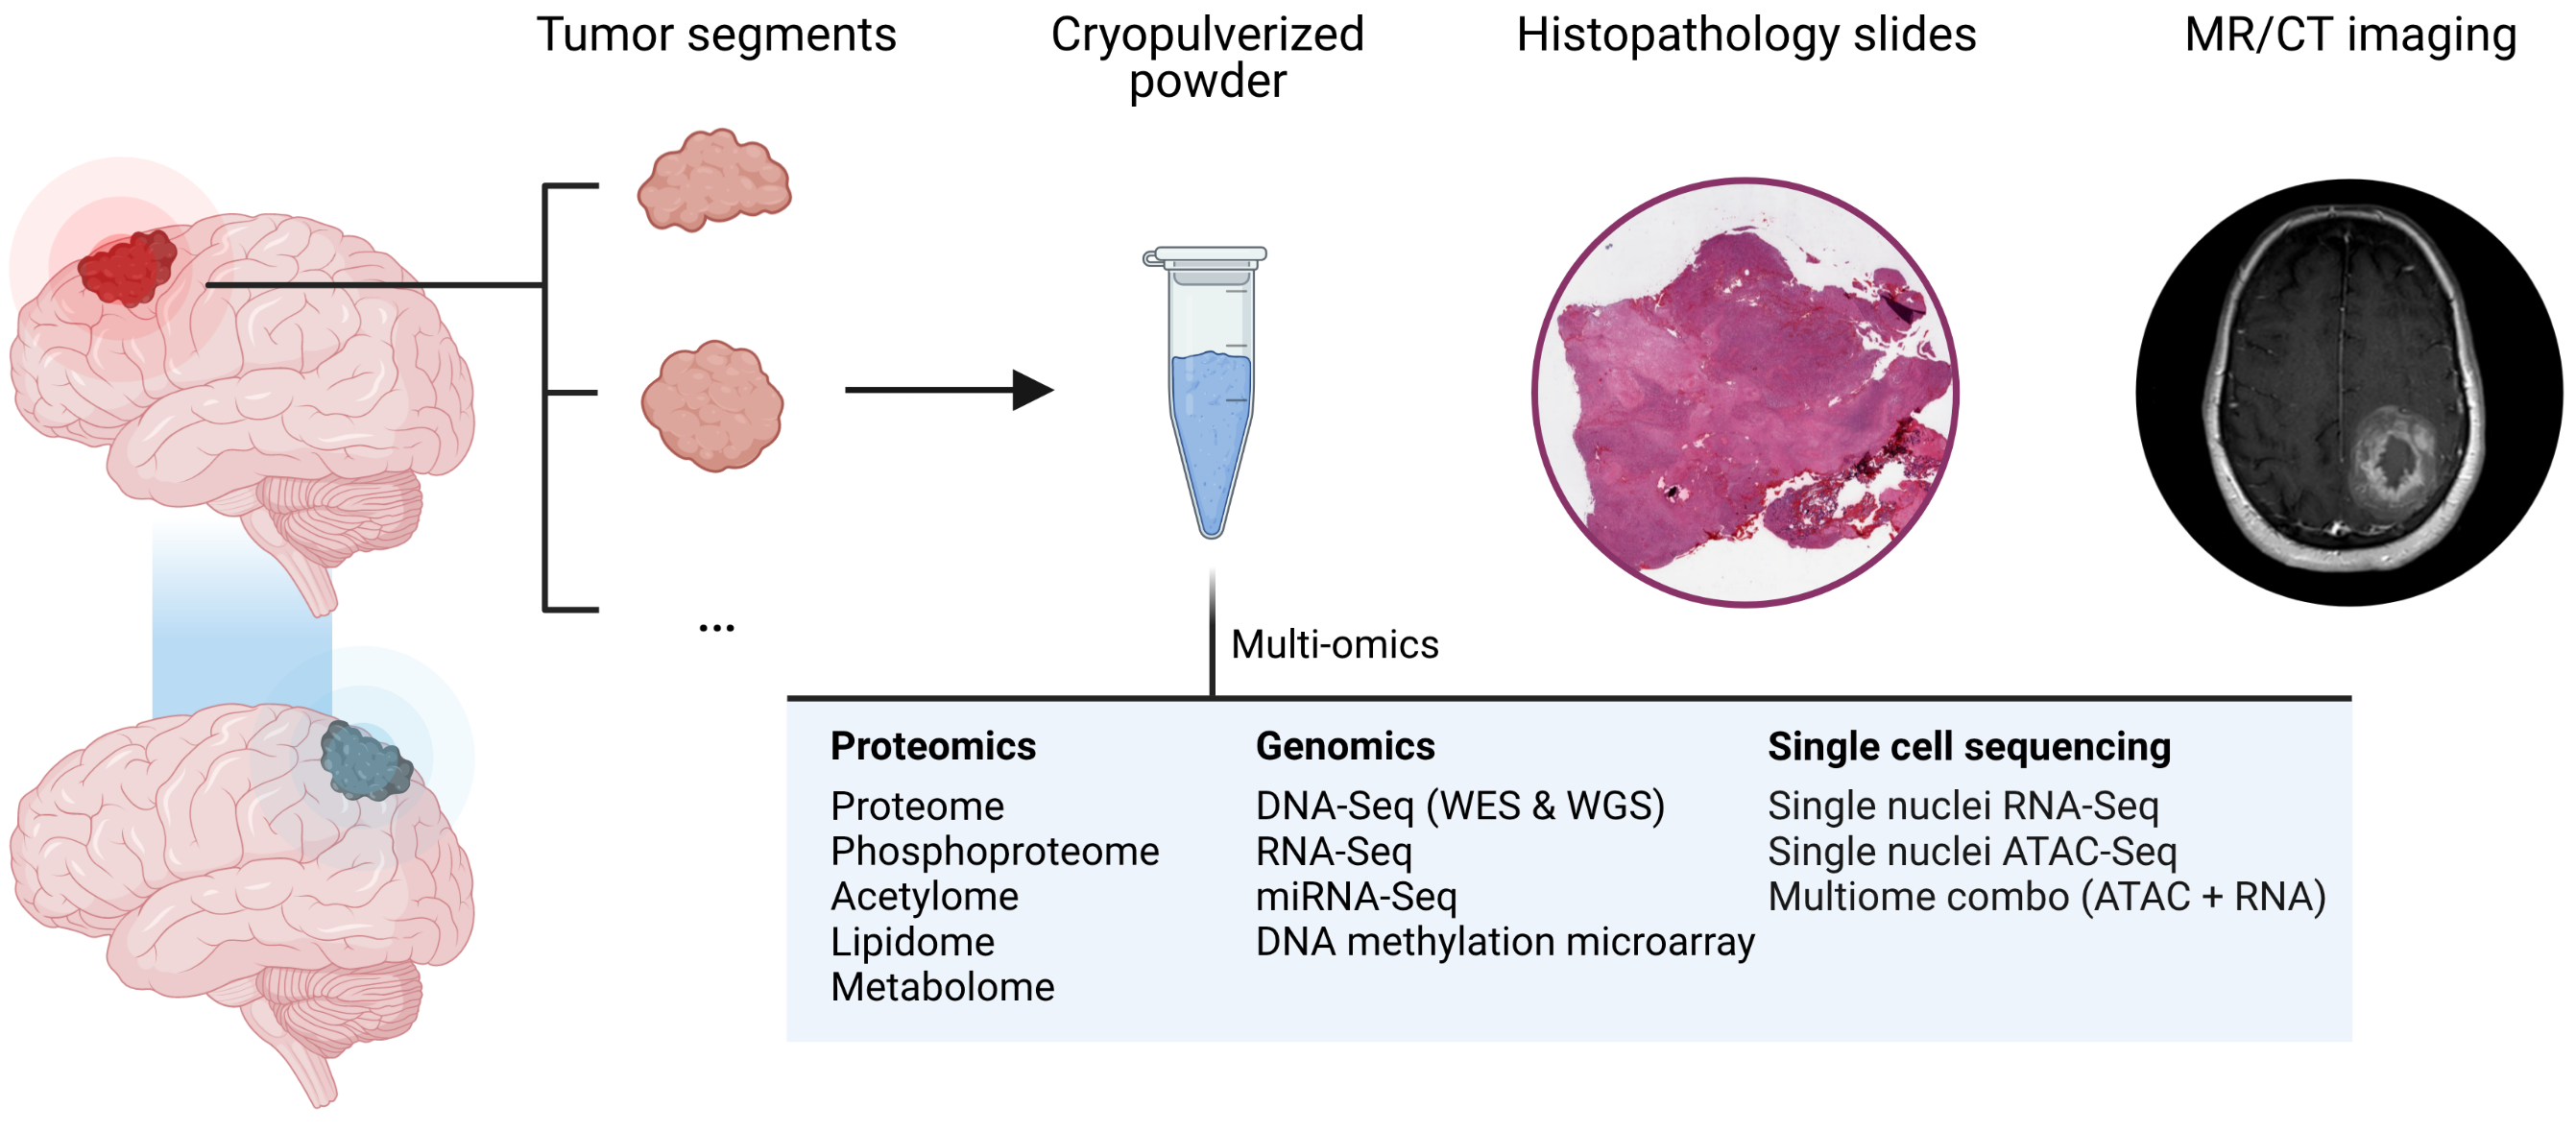
\includegraphics[width=1\linewidth]{figures/chap01_intro/cptac_gbm_multi-omics.png}
    \caption[Overview of the CPTAC GBM data collection and study design.]{%
        Overview of the CPTAC GBM data collection and study design.
        \sourceatright[2em]{\footnotesize Created with BioRender.com}
    }
    \label{fig:intro-cptac-gbm-study-design}
\end{figure}



\defaultlists
